\documentclass[wcp]{jmlr}

\usepackage{enumerate}
\usepackage{bbold}
\usepackage{booktabs}
\usepackage{natbib}
\usepackage[utf8]{inputenc}

 % The following command is just for this sample document:
\newcommand{\cs}[1]{\texttt{\char`\\#1}}


 % change the arguments, as appropriate, in the following:
%\jmlrvolume{1}
%\jmlryear{2014}
%\jmlrworkshop{\textcolor{red}{Neural Connectomics Workshop}}
\jmlrproceedings{}{}

\title{Simple connectome inference from partial correlation statistics in calcium imaging}

\author{Antonio Sutera,
        Arnaud Joly,
        Vincent François-Lavet,
        Aaron Qiu, \\
        Gilles Louppe,
        Damien Ernst,
        Pierre Geurts}

 % Authors with different addresses:
 % \author{\Name{Author Name1} \Email{abc@sample.com}\\
 % \addr Address 1
 % \AND
 % \Name{Author Name2} \Email{xyz@sample.com}\\
 % \addr Address 2
 %}

\editor{Editor's name}
 % \editors{List of editors' names}

\begin{document}

\maketitle

\begin{abstract} In this work, we propose a simple and mathematically
motivated method for the problem of connectome inference in calcium imaging
data. The proposed algorithm is made of two steps. First, processing the raw
signals to detect neural peak activities. Second, inferring the degree of
association between neurons from partial correlation statistics. This paper
summarizes the methodology that led us to win the Connectomics Challenge,
proposes a simplified version of our method and finally discusses our results
with respect to other inference methods. \end{abstract}

\begin{keywords}
Connectomics - Network inference - Partial correlation
\end{keywords}


\section{Introduction}\label{sec:intro}

%%%%%%% !!!!!!!! \textcolor{red}{To improve (style):} !!!! %%%%%%%%
The human brain is a complex biological
organ made of 100 billions of neurons, each connected to 7000 other neurons on
average. Unfortunately, direct observations of the connectome, the wiring
diagram of the brain, is not yet technically feasible. Without being perfect,
calcium imaging currently allows the real-time and simultaneous observation of
neuron activities from thousands of neurons, producing individual time series
representing their fluorescence intensity. From these data, the connectome
inference problem consists in retrieving the synaptic connections between
neurons on the basis of the fluorescence time series. In particular, this
problem is often made difficult because of experimental issues, including
masking effects (making some of the neurons not to be observed or confounded
with others), the low sampling rate of the optical device with respect to the
neural activity speed or the slow decay of fluorescence.
%%%%%%%%%%% !!!!!!!!!!!!!! %%%%%%%%%%%%%%%%

Formally, the connectome can be represented as a directed graph $G=(V,E)$,
where $V$ is a set of $p$ nodes, representing neurons, and $E \subseteq
\left\{(i, j) \in V \times V\right\}$ is a set of edges, representing direct
synaptic connections between neurons. Causal interactions are expressed by the
direction of edges: $(i, j) \in E$ indicates that the state of neuron $j$ might
be caused by the activity of neuron $i$. In those terms,  the connectome
inference problem is formally stated as follows:  \textit{Given the sampled
observations $\{ x^t_i \in \mathbb{R}^{p} | i \in V, t = 1, \dots T \}$ of $p$
neurons for $T$ time intervals, the goal is to infer the set $E$ of connections in $G$.}

In this paper, we present a simplified -- yet nearly as good -- version of the
winning method\footnote{Code available at \url{https://github.com/asutera
/kaggle-connectomics}} of the Connectomics
Challenge\footnote{\url{http://connectomics.chalearn.org}}, as a simple and
theoretically grounded approach based on signal processing techniques and
partial correlation statistics. The paper is structured as follows: Section
\ref{sec:filter} describes the signal processing methods applied on fluorescent
calcium time series; Section \ref{sec:inference} then presents the proposed
approach and its theoretical properties; Section \ref{sec:results} provides an
empirical analysis and comparison with other network inference methods, while
Section \ref{sec:conclusion} finally discusses our work and provides further
research directions. Additionally, Appendix \ref{app:optimized} further
describes, in all details, our actual winning method, giving slightly better
results than the method presented in the paper but highly tuned for the
challenge.


\section{Signal processing} \label{sec:filter}

Under the simplifying assumption that neurons are on-off units, characterized
by short periods of intense activities, or peaks, and longer periods of
inactivity, the first part of our algorithm consists in cleaning the raw
fluorescence data. More specifically, time series are processed using standard
signal processing filters in order to remove noise due light scattering
effects, account for fluorescence  low decay and reduce the importance of
global high activity in the network. The overall process is illustrated on
Figure~\ref{fig:filtered-signal}.


\begin{figure}
\centering
\subfigure[Original]{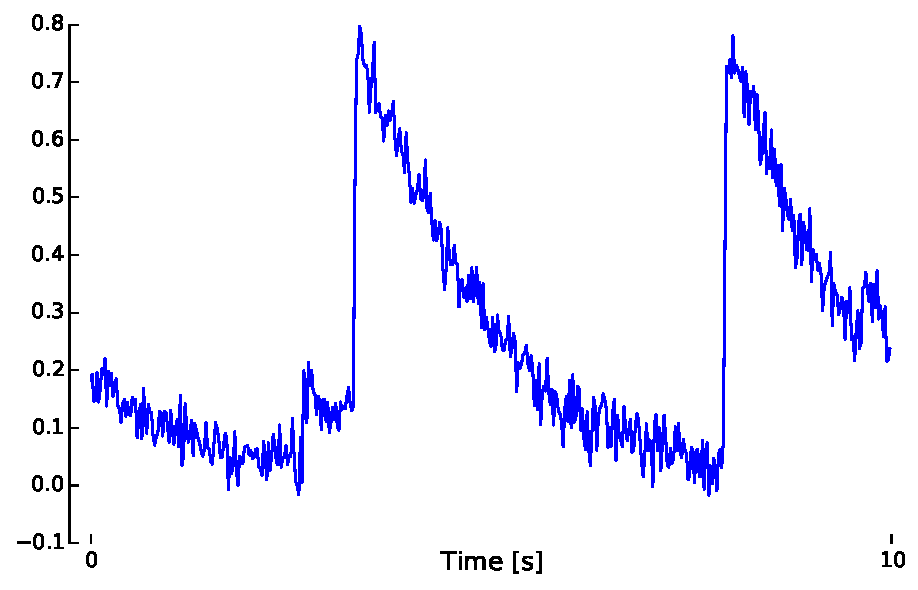
\includegraphics[width=0.3\textwidth]{images/original_curve.pdf} \label{fig:original_curve}}
\subfigure[Low-pass $f_1(x_i^t)$]{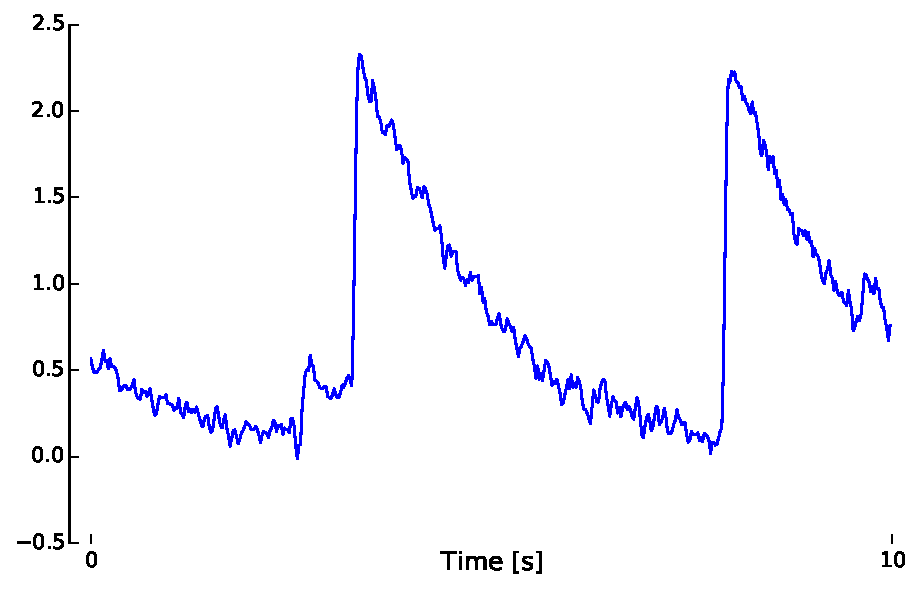
\includegraphics[width=0.3\textwidth]{images/filter_curve.pdf} \label{fig:lp_curve}}\\
\subfigure[High-pass $g(x_i^t)$]{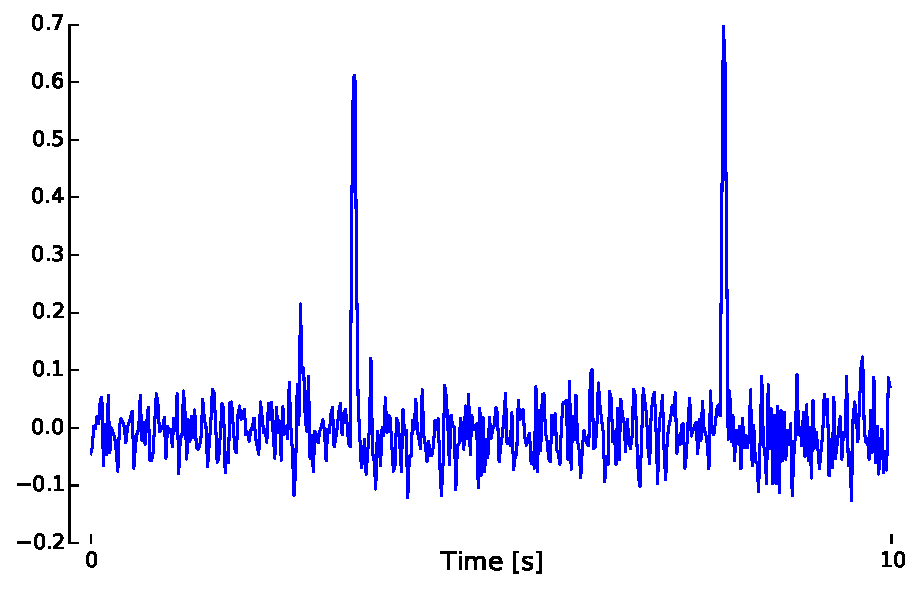
\includegraphics[width=0.3\textwidth]{images/diff_curve.pdf} \label{fig:hp_curve}}
\subfigure[Thresholding $h(x_i^t)$]{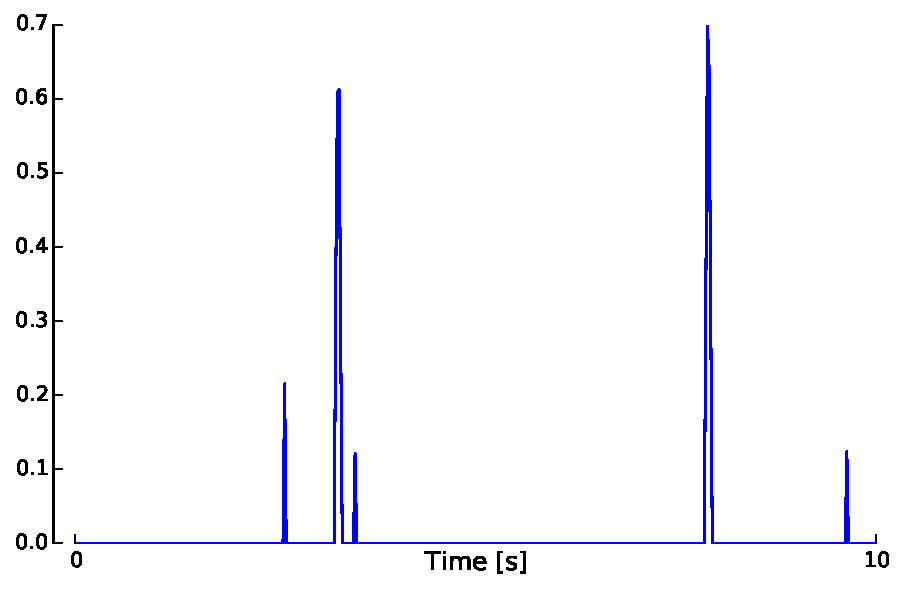
\includegraphics[width=0.3\textwidth]{images/threshold_curve.pdf} \label{fig:threshold_curve}}\\

\subfigure[Weights $w(x_i^t)$]{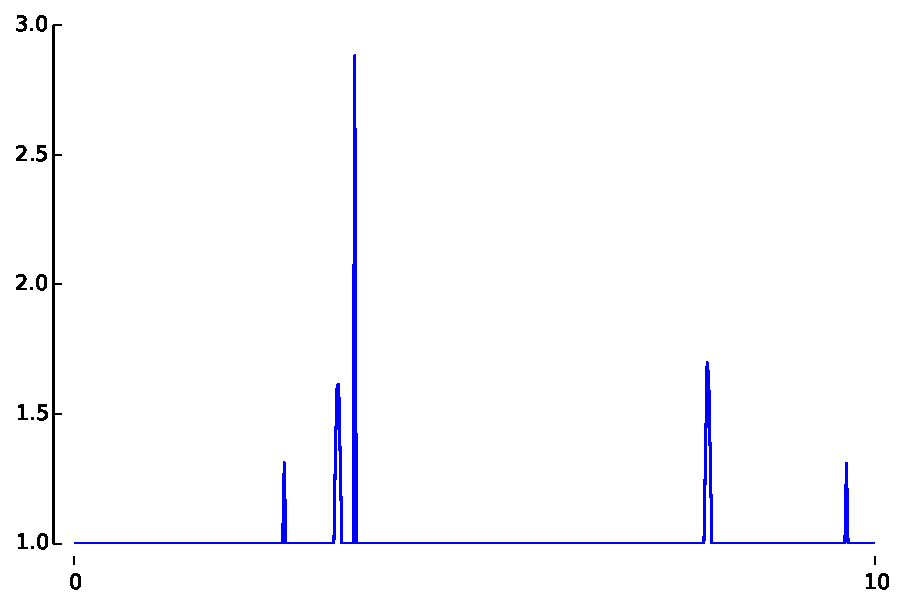
\includegraphics[width=0.3\textwidth]{images/weights_curve.pdf} \label{fig:original_curve}}
\caption{Signal processing process for extracting peaks from the raw fluorescence data.}
\label{fig:filtered-signal}
\end{figure}


% \begin{figure}
% \centering
% 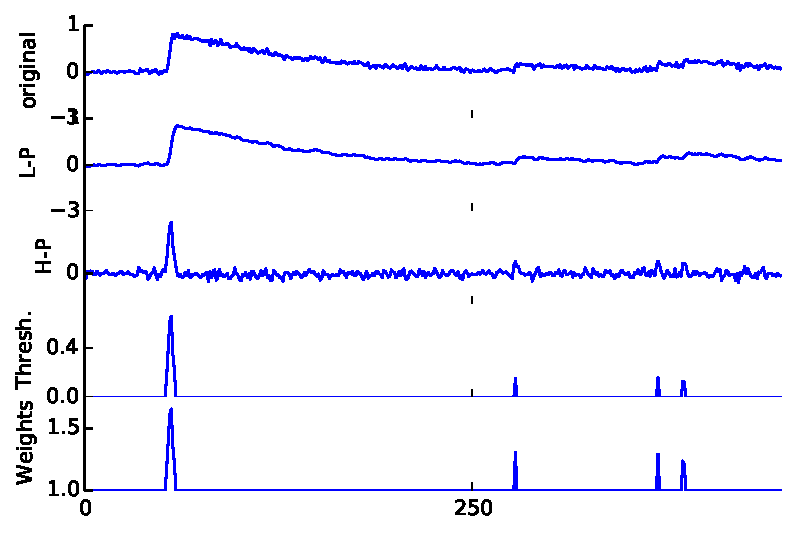
\includegraphics[width=0.4\linewidth]{images/fig_filtering}
% \caption{Signal processing process for extracting peaks from the raw fluorescence data.}
% \label{fig:filtered-signal}
% \end{figure}

As the first plot in Figure~\ref{fig:filtered-signal} illustrates, the raw
fluorescence signal is very noisy due to light scattering artifacts that
ordinarily affects the quality of the recording~\citep{lichtman2011big}.
Accordingly, the first step of our pipeline is to smoothen the signal, using
one the following low-pass filter for filtering out high frequency noise :
\begin{align}
% symmetrical median filter
f_1(x^t_i) &= x^{t-1}_i + x^{t}_i + x^{t+1}_i \label{eq:symetric-median}, \\
% asymmetrical weighted median
f_2(x^t_i) &= 0.4 x^{t-3}_i + 0.6 x^{t-2}_i + 0.8 x^{t-1}_i + x_{t}^i,
\label{eq:weighted-asymetric-median}
\end{align}
where $f_1$x effect is shown in the second plot in the figure.

Considering the short delay of communication between neurons and the slow
decay of fluorescence, the second step of our pipeline consists in identifying
neuron spikes -- characterized by high frequencies -- by filtering out low
frequencies through a high-pass filter, resulting in the third plot of the figure:
\begin{align} % an asymmetrical discrete derivative filter
g(x^{t}_{i}) &= x^{t}_i - x^{t-1}_i. \label{eq:high-pass-filter}
\end{align}

Once the low- and and high-pass filters have been applied, the remaining signal
corresponds to the discrete derivative of the fluorescence time series. To
further filter out small signal variations, mostly due to noise, the third step
consists in a  hard-threshold filter, yielding the fourth plot in the figure:
\begin{align}
h(x^{t}_i) &= x^{t}_i \mathbb{1}(x^{t}_i \geq \tau) \text{ with } \tau > 0.
\end{align}

At this step, the processed signal only contains clean spikes. However, when a
large part of the network is firing, detecting pairwise neuron interactions is a
difficult task. Futhermore, it is even possible that neurons fire because of global high activity, without actual cause (see \cite{stetter2012model}).
% \textcolor{red}{G: say that neurons may fire because of global
% high activity, without any actual cause -- see generator.}
Accordingly, in order to reduce false interaction detection,
peak intensities at time $t$ are regularized by the global activity of all
neurons, thereby reducing the importance of peaks identified during global high activity periods:
\begin{align}
 w(x^{t}_i) &= (x^{t}_i + 1 )^{1 + \frac{1}{\sum_{j} x^{t}_j}}.
\end{align}

In those terms, the full signal processing pipeline of our (simplified)
approach is defined by the composed function $w \cdot h \cdot g \cdot f_1$
(resp. $f_2$ for the winning method).


\section{Connectome inference from partial correlation statistics}
\label{sec:inference}

Let us model the fluorescence indicators of all $p$ neurons as a set of random
variables $X = \{X_1, \dots, X_p\}$ following a joint probability distribution
$P_X$. In the statistical framework, two random variables $X_i$ and $X_j$ are
said to be conditionally independent to a (possibly empty) set of controlling
random variables $Z$, denoted $X_i \perp X_j | Z$, if the joint conditional
probability distribution $P_{X_i, X_j | Z}$ factorizes into $P_{X_i|Z}
P_{X_j|Z}$. In particular, when $X_i$ and $X_j$ are conditionally independent
with respect to all the other variables, denoted $X_i \perp X_j | X^{-i,j}$, then the
observation of $X_i$ given the knowledge of $X^{-i,j}$ provides no information
about $X_j$, and vice-versa. From a graphical point of view and assuming no
hidden variable, this indicates that $X_i$ and $X_j$ do not directly interact
(i.e., $(i,j) \notin E$). By opposition, if $X_i$ and $X_j$ are conditionally
dependent with respect to all other variables, denoted $X_i \not\perp X_j |
X^{-i,j}$, then the observation of one of the two variables provides some
information about the other, therefore highlighting a direct interaction
between the two random variables (i.e., $(i, j) \in E$).

Under the assumption that random variables follow a joint Gaussian
distribution $\mathcal{N}(\mu; \Sigma)$ of mean vector $\mu$ and covariance
matrix $\Sigma$, $X_i$ and $X_j$ are conditionally independent with respect to
the other variables $X^{-i,j}$ if their \textit{partial correlation} statistic
is null~\citep{koller2009probabilistic}, i.e., if
\begin{equation}
\rho_{X_i, X_j | X^{-i,j}} = -\frac{\Sigma^{-1}_{ij}}{\sqrt{\Sigma^{-1}_{ii} \Sigma^{-1}_{jj}}} = 0.
\end{equation}
Conversely, $X_i$ and $X_j$ are conditionally dependent if $\rho_{X_i, X_j | X^{-i,j}} \neq 0$,
where $\rho_{X_i, X_j | X^{-i,j}}$ can now be interpreted as the degree of association
between the two variables (i.e., the larger the value, the stronger the interaction).
Note however that the partial correlation statistic is symmetric (i.e., $\rho_{X_i, X_j | X^{-i,j}} = \rho_{X_j, X_i | X^{-j,i}}$) and therefore does not account for the direction of the interaction.
Together, the partial correlation statistics correspond to the inverse
$\Sigma^{-1}$ of the covariance matrix, also known as the concentration or
precision matrix. Computationally, they can be estimated efficiently in
$O(M^3)$ (instead of $O(p^3)$) from the $M$ first principal components
extracted through PCA~\citep{bishop2006pattern} on the processed data. In our experiments, $M$ is set
to $0.8 p$, thereby allowing us to further filter noise in the data.

To highlight the benefits of measuring the partial dependence conditional to
all other variables, we compare in Section~\ref{sec:results} with the
\textit{Pearson correlation} statistics, which measure instead the linear dependence
between variables, independently of the others. Accordingly, $X_i$ and $X_j$ are
independent if their Pearson correlation statistic is zero, that is if
\begin{equation}
\rho_{X_i,X_j} = \frac{\Sigma_{ij}}{\sqrt{\Sigma_{ii} \Sigma_{jj}}} = 0.
\end{equation}

Finally, let us remark that performance shows to be quite sensitive to the choice
of hyper-parameters in the signal processing pipeline (e.g., $f_1$ or $f_2$ or
the value of the threshold $\tau$). To further improve robustness, the last
step of our method therefore consists in averaging correlation statistics over
various values of the parameters, thereby reducing the variance of our
predictions. In this case, the method is referred to as \textit{Averaged Partial correlation} statistics. Further details are provided in Appendix~\ref{app:optimized}.

\section{Experiments} \label{sec:results}

% Datasets
To assess our method, we focus on the \textit{normal-2} dataset
provided by the organizers of the Connectomics challenge. Experiments
on \textit{normal-1, normal-3, normal-4} show similar trends to
\textit{normal-2} and are presented in the Appendix \textcolor{red}{REF}.
Those datasets have $p=1000$ time series of length $T=179500$ of image
calcium from simulated neuronal networks \citep{stetter2012model}. Those
networks have approximately 15000 edges.

% Metrics : ROC AUC and AUPRC
In supervised learning terms, the network inference task can be viewed as a
binary classification task where one has to correctly classify the presence or
the absence of edges of the graph. We assess the accuracy of the network
inference method using the area under the ROC curve (AUROC) and the area under
the precision-recall curve (AUPRC) \citep{schrynemackers2013protocols}. Since
neurons are not self-connected ($(i, i) \not \in E, \forall i \in V$) and some
inference methods could give maximal scores to those edges, e.g. Pearson
correlation, those elements are set to have minimal connectivity score prior
assessment.

We will compare our approach to the Pearson correlation (see Section
\ref{sec:inference}), the generalized transfer entropy (GTE) and GENIE3.
\begin{itemize}
\item \textbf{GTE} \citep{stetter2012model}
, the baseline of the challenge, measures for all pairs of
neurons $i$ and $j$ the reduction of uncertainty in predicting future values of
$i$ given the observation of the time series of the neuron $j$
conditionally to the observation of past time series of neuron $i$,
whenever the average fluorescence is over a conditioning level.
Pre-processing and conditioning level were set to reproduce baseline of the
challenge.

\item \textbf{GENIE3} \citep{huynhthu2010inferring} translates the inference
of the network of $p$ neurons into $p$ supervised learning tasks. For each
task, the fluorescence of a neuron is predicted from the fluorescence of all
other neurons using a tree based ensemble such as random forest
\citep{breiman2001random}. The tree ensemble associates a variable importance
score \citep{louppe2013understanding} to each neuron used in the predictions,
which is used as a degree of associate. The following parameters are used
$10000$ trees, $\log_2{p}$ variables are randomly selected to split tree nodes
and the maximal tree depth is constrained to 1, 2 or 3. \end{itemize}


\subsection*{Partial correlation improves over state-of-the-art methods}

Figure \ref{fig:curves} shows the ROC curve  and precision-recall curve
for correlation, GTE and partial correlation on the \textit{normal-2}
dataset. The partial correlation outperforms other state-of-the-art methods
by at least factor of 2 in AUPRC reaching $0.347$ and an increased of $0.05$ in
AUROC. Two reasons might explain such differences: (i) among
those methods only the partial correlation makes the distinction between
direct and indirect connections, (ii) the simulated network from the
\citep{stetter2012model} generator or the neural network in general could be
reduced to a linear model after pre-processing. Those results is obviously
generalized over the other datasets see Appendix \textcolor{red}{REF}.

\begin{figure}[bth]
\centering
\subfigure[ROC curves]{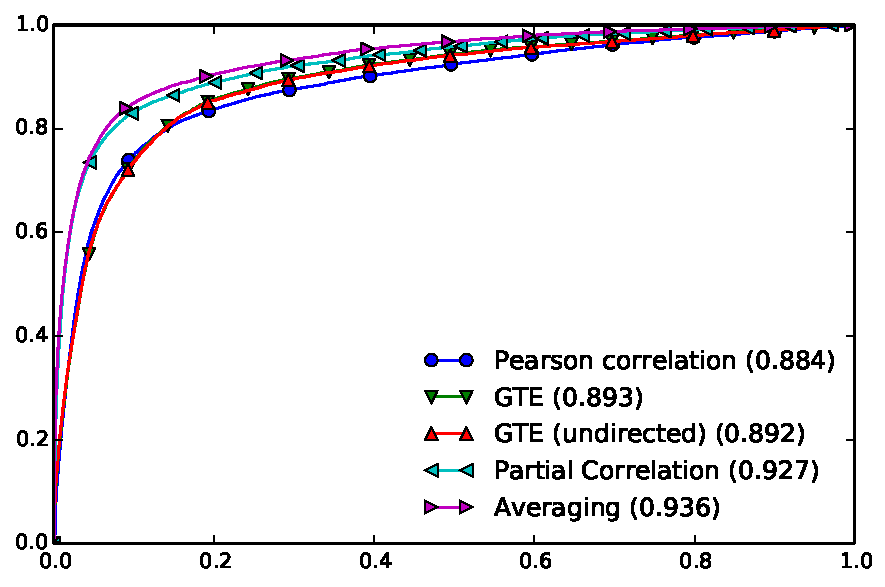
\includegraphics[width=0.45\textwidth]{images/curve_roc} \label{fig:roc_curve}}
\subfigure[Precision-recall curves]{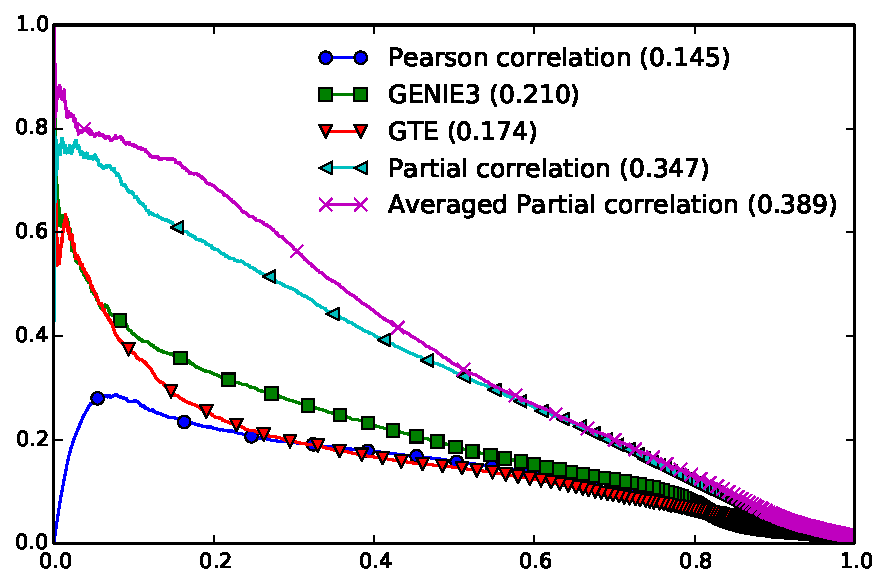
\includegraphics[width=0.45\textwidth]{images/curve_pr} \label{fig:pr_curve}}
\caption{The weighted average of partial correlation matrix, winning approach
         of the challenge, yields better than AUROC and AUPRC than all
         other state-of-the-art methods. (parameters: $\tau=0.11$ except for
         averaged partial correlation method, partial correlation used
         filter $f_1$). }
\label{fig:curves}
\end{figure}



\textcolor{red}{AJ: GENI3 is not on the figure}
As it can also be seen on Figure \ref{fig:curves}, the GENIE3 performance
increases with deeper trees in addition to be computationally feasible. The
reason is twofold. First, the deeper the tree, the larger is the conditioning.
As it was observed in the comparison between correlation and partial
correlation, it screens indirect links in the inferred network. Second, the
number of small trees need to be much higher than deep trees in order to
observe - and evaluate - all pairs.  However, as suggested by
\cite{louppe2014understanding}, limiting the maximal depth of trees may help
to reduce the misestimation bias in variable importance computing, i.e.
inferring the strength of a link. Therefore a trade-off of the maximal depth
may give the best of both worlds.

% Opt: obviously when parameters are tuned/optimized, it's slightly better -->
% see appendix for a full description of the method


% \begin{table}
% \small
% \centering
% \begin{tabular}{@{}l *{8}{c}@{}}
%   & \multicolumn{4}{c}{AUROC} & \multicolumn{4}{c}{AUPRC} \\
% \cmidrule(r){2-5}\cmidrule(r){6-9}
% Methods $\backslash$ normal- & 1 & 2 & 3 & 4 & 1 & 2 & 3 & 4 \\
% \hline \hline
% % Directivity \textcolor{red}{appendix?} & 0.535 & 0.526 & 0.533 & 0.535 & 0.012 & 0.012 & 0.012 & 0.012 \\
% GENIE3 (depth = 1)     &  & & & & & & & \\
% GENIE3 (depth = 2)     &  & & & & & & & \\
% GENIE3 (depth = 3)     &  & & & & & & & \\
% GTE                    &  & & & & & & & \\
% % Our approach + dir  \textcolor{red}{appendix?}   & 0.944 & 0.943 & 0.942 & 0.940 & 0.404 & 0.405 & 0.399 & 0.389 \\
% \end{tabular}
% \caption{TODO (network are undirected)}
% \label{tab:tab2}
% \end{table}




\subsection*{Area under the ROC curve a poor metric for network inference}

The best method only infers the \textbf{undirected} network by giving the same
degree of association to both edges $(i,j)$ and $(j,i)$. This is quite
surprising considering the problem statement. Trying to direct links could be
more penalizing than rewarding. For example, symmetrizing the degree of
association matrix does not necessarily degrade AUPRC and AUROC.


If the inferred network corresponds to the undirected network, it would
already yield high AUROC score for instance $\approx 0.996$ on
\textit{normal-1}. Infering edge directivity is likely to be counter-
productive or yield small gain. By contrast, the same experiment with AUPRC
would yield to a score of $\approx 0.789$ on \textit{normal-1}. Thus inferring
correctly directivity would be more rewarding in AUPRC term.



% Interestingly, methods that takes into account directivity, namely GTE and
% GENIE3, improve their AUROC and AUPRC by giving the same way to directed edges.
% (in particular see GTE and GTE(undirected) in Figure \ref{fig:pr_curve}
% \textcolor{red}{AJ: Figure \ref{fig:curves}  contradicts this message,
% especially pr-curve. AS:And now?} and Table \ref{tab:tab1} in Appendix \textcolor{red}{REF}).
% Trying to detect the link direction is more penalizing than rewarding.

The area under the ROC curve is not consistent metric
with respect to the problem statement. A clear hierarchy is also difficult to
derive based on ROC curve of Figure \ref{fig:roc_curve}. We advice to avoid the AUROC
for the assessment of network inference method. An alternative metric would
be the area under the precision-recall curve (AUPRC). Those
conclusions are in line with \cite{schrynemackers2013protocols}.


\section{Conclusions} \label{sec:conclusion}


% Possible extensions
% partial autocorrelation function (sometimes "partial correlation function")
% conditional independence test
% Speak about the complexity and parallelization of the methods



In this paper, we present the winning method of the Connectomics challenge.
This approach is simple and theoretically grounded. We also evaluate the method
in a more detailed way and perform a comparison with other inference methods.
We also discuss the relevance of the metric used in the challenge.

In the discussion, we give hints about limiting the depth of trees in the
GENIE3 method to infer the network. It should be interesting to see if there
is a optimum value for the maximal depth. And of course, it may also rewarding
to increase considerably the number of trees to get more stable predictions.

In previous study \citep{shipley2002cause}, it has been suggested to
consider correlation coefficients of all possible orders,
i.e. conditioned on every subsets of the set of $p-2$ other variables. This
would take into account multiple indirect paths between a given pair of
variables. Instead of considering only the highest order, it may be useful to
study with accuracy the inferred network at all orders. In this case, it may not
be very relevant but interesting in case of dynamical networks.

As we mentioned, in order to maximize the ROC AUC, it was not necessary to
discover causal relationships. It may be, in future works, promising to focus
on that particular topic.


\section*{Acknowledgments}
A. Joly and G. Louppe are research fellows of
the FNRS, Belgium.  A. Sutera is recipient of
a F.R.I.A. fellowship of F.R.S.-FNRS, Belgium.
This work is supported by PASCAL2 and the IUAP DYSCO, initiated by the
Belgian State, Science Policy Office.



\newpage
\clearpage

% We allow the bibliography to be added on top of the 6 pages.
% Supplementary material may be added in the form or a URL pointed to from
% the paper.
\bibliography{references}

\newpage
\clearpage

\appendix


\section{An optimized version of the algorithm to win the challenge}
\label{app:optimized}


The algorithm propose in sections \ref{sec:filter} and \ref{sec:inference} has been optimized at its extreme limit to win the challenge. In this section, we will describe the full tuned algorithm and present some results.

Note that our parameter tuning was mainly
done on the \textit{normal-1} dataset and partly on \textit{normal-4} dataset,
therefore it may justify why these networks are better retrieved despite the
fact that some might be simpler to infer.

% Introduce a custom solution to make the Y matrix asymmetric
% Introduce directivity
\textcolor{red}{Est-ce qu'on ne le ferait pas passer dans l'appendice B? Ou du moins l'équation?}
Since partial correlation is a symmetric measure, the causal mechanism behind the
interaction ($A$ directly causes $B$, $B$ directly causes $A$ or both) can not
be directly inferred\footnote{Also note that two other causal mechanisms might be
implied while having a non-zero partial coefficient: (i) a pair of variables
is induced by a common (hidden) variable; (ii) $A$ (respectively $B$) is
conditionally correlated to a hidden variable affecting $B$ (resp. $A$)
\citep{de2004discovery}.}.
In order to retrieve causal information, we developed an
heuristics based on the following observation. The rise of fluorescence
indicates the activation of a neuron $i$. If a neuron $j$ have also
an increased of fluorescence after a slight delay, this could have been
caused by the neuron $i$. Thus, we count whenever
such events occurred between consecutive time steps
\[
\hat{Z}: z_{ij} = \sum_{t=1}^{T - 1}
    \mathbb{1}(x_j^{t+1} - x_i^t \in \left[f_1, f_2 \right]) -
    \mathbb{1}(x_i^{t+1} - x_j^t \in \left[f_1, f_2 \right]), \forall i, j \in V
\]
where $f_1$ and $f_2$ are parameters of the method.
Finally, the weighted average of correlation matrices is combined with $Z$ such
that $Z$ has a contribution of $0.3\%$ to the prediction of an edge.

% For the directory method, only filters defined by Equations
% \ref{eq:low-pass}, \ref{eq:high-pass} and \ref{eq:hard-treshold-filter} were
% used.


\section{Extended results}

\begin{table}
\small
\centering
\begin{tabular}{@{}l *{8}{c}@{}}
  & \multicolumn{4}{c}{AUROC} & \multicolumn{4}{c}{AUPRC} \\
\hline \hline
Methods $\backslash$ normal- & 1 & 2 & 3 & 4 & 1 & 2 & 3 & 4 \\
\hline \hline
% Directivity \textcolor{red}{appendix?} & 0.535 & 0.526 & 0.533 & 0.535 & 0.012 & 0.012 & 0.012 & 0.012 \\
Pearson correlation    & 0.886 & 0.884 & 0.891 & 0.877 & 0.153 & 0.145 & 0.170 & 0.132 \\
GENIE3 (depth = 1)     & 0.878 & & & & 0.184 & & & \\
GENIE3 (depth = 2)     & 0.889 & & & & 0.217 & & & \\
GENIE3 (depth = 3)     & & & & & & & & \\
GTE                    & 0.890 & 0.893 & 0.894 & 0.873 & 0.171 & 0.174 & 0.197 & 0.142 \\
Partial correlation    & 0.930 &  0.927 &  0.926 &  0.923& 0.363  & 0.347 &  0.346 & 0.328 \\
Partial correlation (avg.) & 0.938 & 0.936 & 0.936 & 0.932& 0.391 & 0.389 & 0.385 & 0.374\\
% Our approach simple + dir & 0.939 & 0.936 & 0.937 & 0.933& 0.392 & 0.390 & 0.386 & 0.375\\
Partial correlation (opt.) & 0.932 & 0.931 & 0.930 & 0.928 & 0.364 & 0.366 & 0.359 & 0.344 \\
Our approach (opt. \& avg.)    & 0.943 & 0.942 & 0.942 & 0.939 & 0.403 & 0.404 & 0.398 & 0.388 \\
% Our approach + dir  \textcolor{red}{appendix?}   & 0.944 & 0.943 & 0.942 & 0.940 & 0.404 & 0.405 & 0.399 & 0.389 \\
\end{tabular}
\caption{TODO}
\label{tab:tab1}
\end{table}


\section{Supplementary results}

\begin{table}[htbp]
\centering
\caption{Correlation (ROC). Improvement of each stage of our approach. Note that we choose the
         \textit{best} threshold (\textcolor{red}{for now 0.11}) for stages 1 to 4.}
\begin{tabular}{*{5}{l}}
\toprule
Stage               & normal-1 & normal-2 & normal-3 & normal-4 \\
\midrule
Nothing             & 0.681 & 0.699 & 0.683 & 0.681\\
Weights             & 0.695 & 0.713 & 0.697 & 0.694\\
H-T                 & 0.876 & 0.873 & 0.877 & 0.869\\
H-T + Weights       & 0.886 & 0.884 & 0.891 & 0.877\\
P-P                 & 0.857 & 0.850 & 0.843 & 0.832\\
P-P + Weights       & 0.826 & 0.823 & 0.817 & 0.799\\
\bottomrule
\end{tabular}
\end{table}

\begin{table}[htbp]
\centering
\caption{Correlation (P-R). Improvement of each stage of our approach. Note that we choose the
         \textit{best} threshold (\textcolor{red}{for now 0.11}) for stages 1 to 4.}
\begin{tabular}{*{5}{l}}
\toprule
Stage               & normal-1 & normal-2 & normal-3 & normal-4 \\
\midrule
Nothing             & 0.028 & 0.028 & 0.025 & 0.026\\
Weights             & 0.031 & 0.030 & 0.027 & 0.028\\
H-T                 & 0.143 & 0.128 & 0.150 & 0.129\\
H-T + Weights       & 0.153 & 0.145 & 0.170 & 0.132\\
P-P                 & 0.100 & 0.087 & 0.079 & 0.083\\
P-P + Weights       & 0.079 & 0.071 & 0.067 & 0.064\\
\bottomrule
\end{tabular}
\end{table}

\begin{table}[htb]
\centering
\caption{Comparison (P-R) with other methods (for now, $t = 0.11$)}
\begin{tabular}{*{5}{l}}
\toprule
Methods             & normal-1 & normal-2 & normal-3 & normal-4 \\
\midrule
Correlation (best)         & 0.153 & 0.145 & 0.170 & 0.132 \\
Partial correlation (best) & 0.364 & 0.366 & 0.359 & 0.344 \\
Our approach (best)        & 0.403 & 0.404 & 0.398 & 0.388 \\
GENIE3                     & & & & \\
GTE                        & 0.171 & 0.174 & 0.197 & 0.142 \\
Directivity                & 0.012 & 0.012 & 0.012 & 0.012 \\
Our approach + dir         & 0.404 & 0.405 & 0.399 & 0.389 \\
\bottomrule
\end{tabular}
\end{table}

\begin{table}[htb]
\centering
\caption{Inverse correlation (ROC). Improvement of each stage of our approach. Note that we choose the
         \textit{best} threshold (\textcolor{red}{for now 0.11}) for stages 1 to 4.}
\begin{tabular}{*{5}{l}}
\toprule
Stage               & normal-1 & normal-2 & normal-3 & normal-4 \\
\midrule
Nothing             & 0.777 & 0.767 & 0.772 & 0.774 \\
PCA                 & 0.780 & 0.770 & 0.776 & 0.777 \\
Weights             & 0.780 & 0.769 & 0.776 & 0.777 \\
Weights + PCA       & 0.783 & 0.772 & 0.779 & 0.780 \\
H-T                 & 0.893 & 0.891 & 0.891 & 0.886 \\
H-T + PCA           & 0.894 & 0.892 & 0.891 & 0.886 \\
H-T + Weights       & 0.899 & 0.897 & 0.896 & 0.891 \\
H-T + Weights + PCA & 0.900 & 0.898 & 0.896 & 0.892 \\
P-P                 & 0.925 & 0.925 & 0.924 & 0.923 \\
P-P + PCA           & 0.926 & 0.926 & 0.925 & 0.923 \\
P-P + Weights       & 0.931 & 0.930 & 0.928 & 0.927 \\
P-P + Weights + PCA & 0.932 & 0.931 & 0.930 & 0.928 \\
Averaging (PCA)     & 0.943 & 0.942 & 0.942 & 0.939 \\
Stacking            & 0.944 & 0.943 & 0.942 & 0.940 \\
\bottomrule
\end{tabular}
\end{table}

\begin{table}[htb]
\centering
\caption{Inverse correlation (P-R). Improvement of each stage of our approach. Note that we choose the
         \textit{best} threshold (\textcolor{red}{for now 0.11}) for stages 1 to 4.}
\begin{tabular}{*{5}{l}}
\toprule
Stage               & normal-1 & normal-2 & normal-3 & normal-4 \\
\midrule
Nothing             & 0.070 & 0.064 & 0.068 & 0.072\\
PCA                 & 0.076 & 0.070 & 0.075 & 0.079\\
Weights             & 0.074 & 0.067 & 0.072 & 0.076\\
Weights + PCA       & 0.080 & 0.073 & 0.079 & 0.083\\
H-T                 & 0.264 & 0.260 & 0.269 & 0.241\\
H-T + PCA           & 0.266 & 0.263 & 0.273 & 0.244\\
H-T + Weights       & 0.280 & 0.273 & 0.281 & 0.251\\
H-T + Weights + PCA & 0.284 & 0.278 & 0.285 & 0.255\\
P-P                 & 0.322 & 0.324 & 0.323 & 0.312\\
P-P + PCA           & 0.347 & 0.352 & 0.355 & 0.341\\
P-P + Weights       & 0.333 & 0.334 & 0.327 & 0.313\\
P-P + Weights + PCA & 0.364 & 0.366 & 0.359 & 0.344\\
Averaging           & 0.403 & 0.404 & 0.398 & 0.388\\
Stacking            & 0.404 & 0.405 & 0.399 & 0.389\\
\bottomrule
\end{tabular}
\end{table}


\section{Signal processing highly improves performance}


On Table \ref{tab:tab3}, it can be seen that each step of our approach globally
improves the score on both metrics. However, processing, weights and averaging
(respectively denoted as $P$,$W$ and $Averaging$ in Tab.\ref{tab:tab3}) as
described in Section \ref{sec:filter} are the key steps of our algorithm.

It also appears that the averaging over the low-pass filter designs and the
threshold values increases significantly the quality of the inferred network
according to both metrics.

% Explaining the method (thèse de Gilles)
% Avg.: Averaging over the threholds and L-P filters improves a lot both metrics.
% Averaging

%% Depth -- Gilles chapitre 7
% Genie3 : better in auprc while worse in auroc than GTE. Why?
% Genie3 : "Conditioning" better and better but need a lot of trees

\begin{table}[tbh]
\centering
\small
\begin{tabular}{@{}l *{8}{c}@{}}
\hline
  & \multicolumn{4}{c}{AUROC} & \multicolumn{4}{c}{AUPRC} \\
\hline
Methods $\backslash$ normal- & 1 & 2 & 3 & 4 & 1 & 2 & 3 & 4 \\
No  filtering       & 0.777 & 0.767 & 0.772 & 0.774 & 0.070 & 0.064 & 0.068 & 0.072\\
P                   & 0.925 & 0.925 & 0.924 & 0.923 & 0.322 & 0.324 & 0.323 & 0.312\\
P + W               & 0.931 & 0.930 & 0.928 & 0.927 & 0.333 & 0.334 & 0.327 & 0.313\\
P + W + PCA         & 0.932 & 0.931 & 0.930 & 0.928 & 0.364 & 0.366 & 0.359 & 0.344\\
Averaging           & 0.943 & 0.942 & 0.942 & 0.939 & 0.403 & 0.404 & 0.398 & 0.388\\
%Averaging + Directivity & 0.944 & 0.943 & 0.942 & 0.940 & 0.404 & 0.405 & 0.399 & 0.389\\
\end{tabular}
\caption{TODO \textcolor{red}{version simple!!}}
\label{tab:tab3}
\end{table}

%% Talk about filters future and past

\end{document}

